% coding:utf-8

% Ausführen in R: 
% Sweave("C:/Daten/Daniel/studium/git_repo/sem2/stoc/sw10/sw10_5.Rnw",encoding='UTF-8')

\section{Aufgabe 5}

\subsection{a}
\begin{Schunk}
\begin{Sinput}
> plot(anscombe[,'x1'],anscombe[,'y1'])
> abline(lm(anscombe[,'y1']~anscombe[,'x1']),col='green')
\end{Sinput}
\end{Schunk}
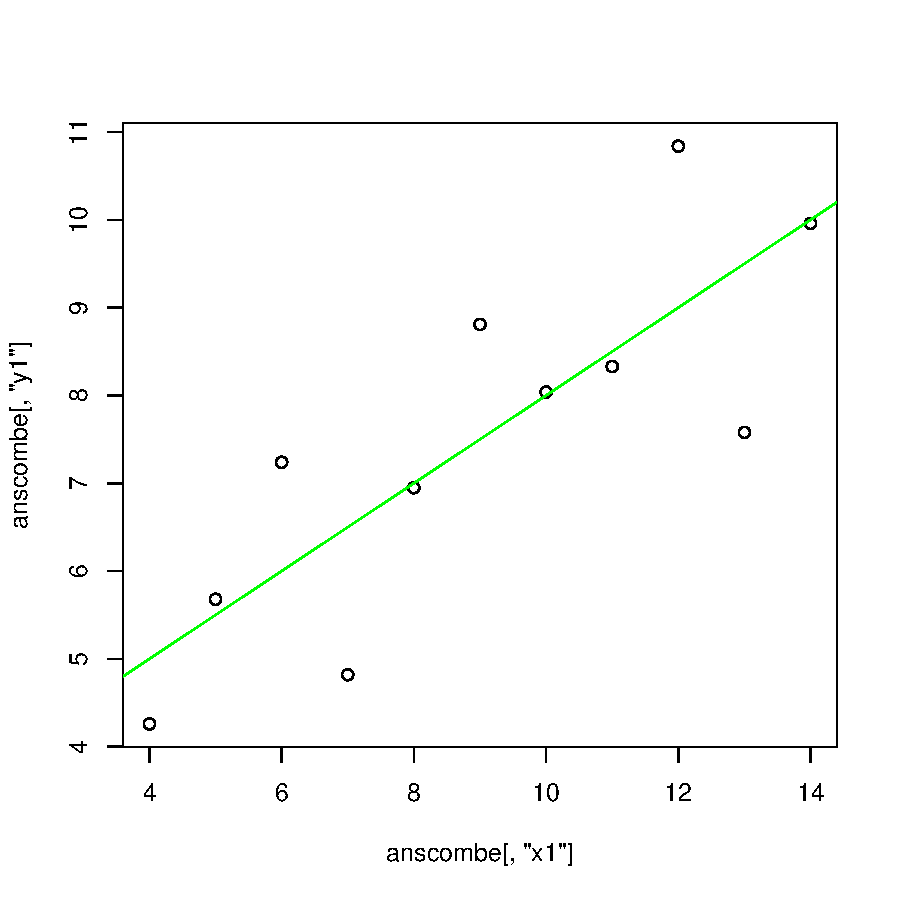
\includegraphics{sw11_5-001}
\begin{Schunk}
\begin{Sinput}
> plot(anscombe[,'x2'],anscombe[,'y2'])
> abline(lm(anscombe[,'y2']~anscombe[,'x2']),col='green')
\end{Sinput}
\end{Schunk}
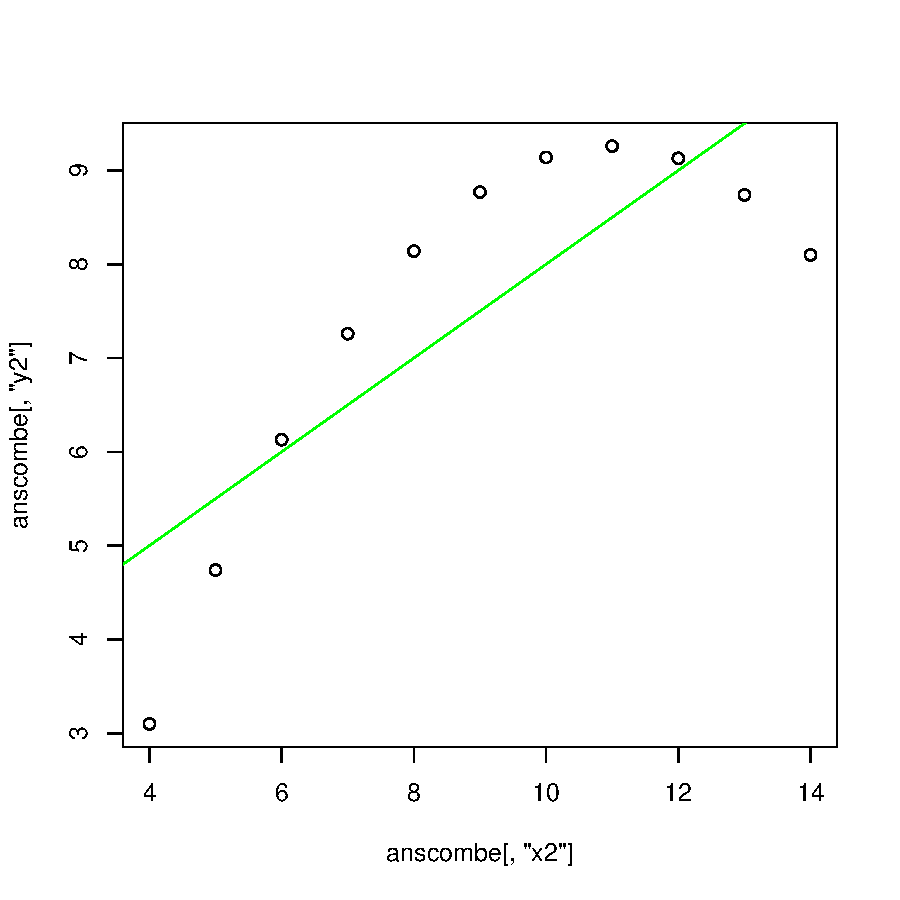
\includegraphics{sw11_5-002}
\begin{Schunk}
\begin{Sinput}
> plot(anscombe[,'x3'],anscombe[,'y3'])
> abline(lm(anscombe[,'y3']~anscombe[,'x3']),col='green')
\end{Sinput}
\end{Schunk}
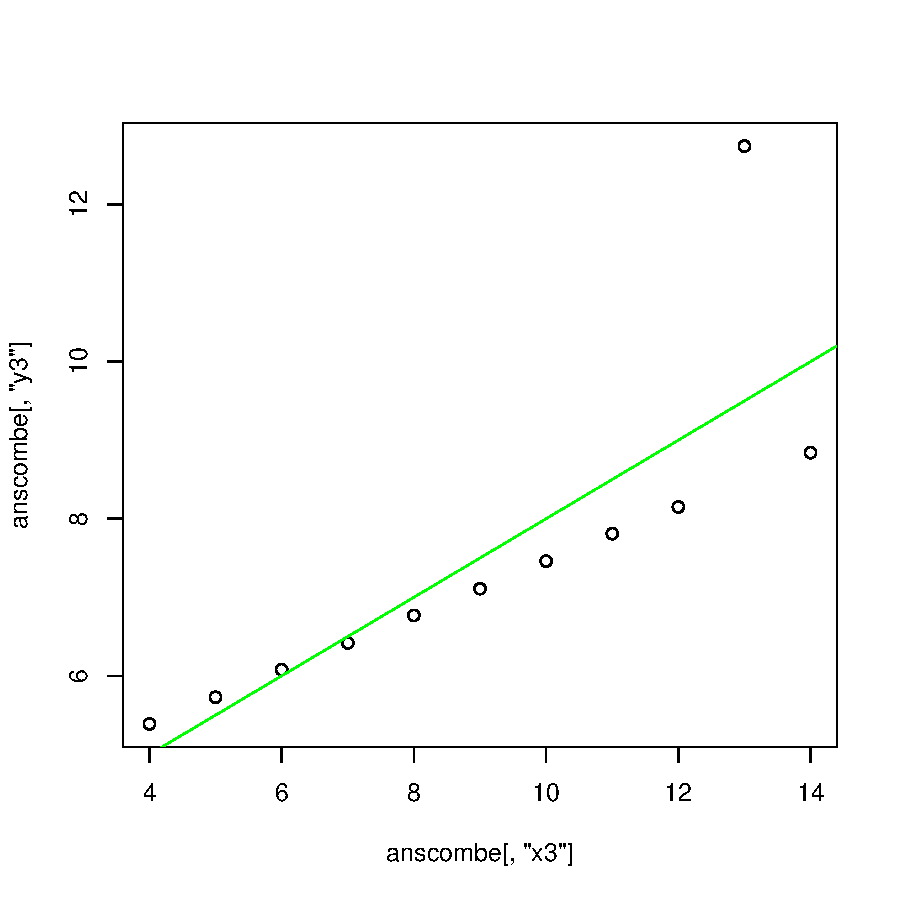
\includegraphics{sw11_5-003}
\begin{Schunk}
\begin{Sinput}
> plot(anscombe[,'x4'],anscombe[,'y4'])
> abline(lm(anscombe[,'y4']~anscombe[,'x4']),col='green')
\end{Sinput}
\end{Schunk}
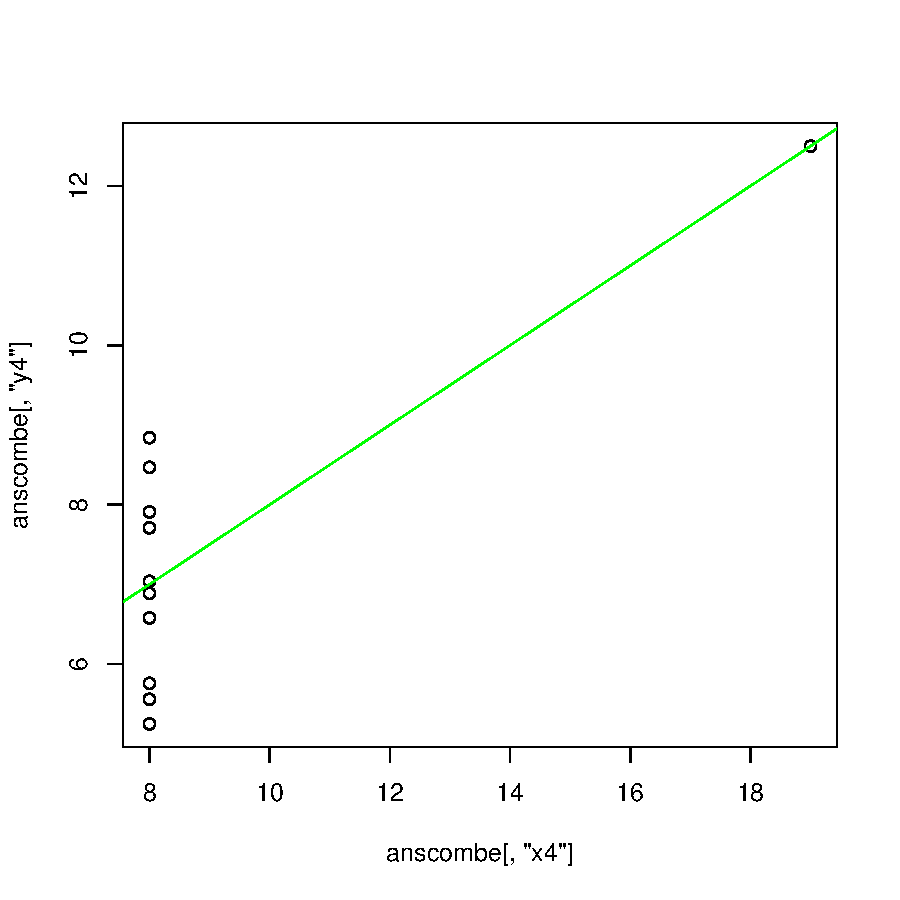
\includegraphics{sw11_5-004}

\subsection{b}
\begin{Schunk}
\begin{Sinput}
> summary(lm(anscombe[,'y1']~anscombe[,'x1']))
\end{Sinput}
\begin{Soutput}
Call:
lm(formula = anscombe[, "y1"] ~ anscombe[, "x1"])

Residuals:
     Min       1Q   Median       3Q      Max 
-1.92127 -0.45577 -0.04136  0.70941  1.83882 

Coefficients:
                 Estimate Std. Error t value Pr(>|t|)   
(Intercept)        3.0001     1.1247   2.667  0.02573 * 
anscombe[, "x1"]   0.5001     0.1179   4.241  0.00217 **
---
Signif. codes:  0 ‘***’ 0.001 ‘**’ 0.01 ‘*’ 0.05 ‘.’ 0.1 ‘ ’ 1 

Residual standard error: 1.237 on 9 degrees of freedom
Multiple R-squared: 0.6665,	Adjusted R-squared: 0.6295 
F-statistic: 17.99 on 1 and 9 DF,  p-value: 0.00217 
\end{Soutput}
\begin{Sinput}
> summary(lm(anscombe[,'y2']~anscombe[,'x2']))
\end{Sinput}
\begin{Soutput}
Call:
lm(formula = anscombe[, "y2"] ~ anscombe[, "x2"])

Residuals:
    Min      1Q  Median      3Q     Max 
-1.9009 -0.7609  0.1291  0.9491  1.2691 

Coefficients:
                 Estimate Std. Error t value Pr(>|t|)   
(Intercept)         3.001      1.125   2.667  0.02576 * 
anscombe[, "x2"]    0.500      0.118   4.239  0.00218 **
---
Signif. codes:  0 ‘***’ 0.001 ‘**’ 0.01 ‘*’ 0.05 ‘.’ 0.1 ‘ ’ 1 

Residual standard error: 1.237 on 9 degrees of freedom
Multiple R-squared: 0.6662,	Adjusted R-squared: 0.6292 
F-statistic: 17.97 on 1 and 9 DF,  p-value: 0.002179 
\end{Soutput}
\begin{Sinput}
> summary(lm(anscombe[,'y3']~anscombe[,'x3']))
\end{Sinput}
\begin{Soutput}
Call:
lm(formula = anscombe[, "y3"] ~ anscombe[, "x3"])

Residuals:
    Min      1Q  Median      3Q     Max 
-1.1586 -0.6146 -0.2303  0.1540  3.2411 

Coefficients:
                 Estimate Std. Error t value Pr(>|t|)   
(Intercept)        3.0025     1.1245   2.670  0.02562 * 
anscombe[, "x3"]   0.4997     0.1179   4.239  0.00218 **
---
Signif. codes:  0 ‘***’ 0.001 ‘**’ 0.01 ‘*’ 0.05 ‘.’ 0.1 ‘ ’ 1 

Residual standard error: 1.236 on 9 degrees of freedom
Multiple R-squared: 0.6663,	Adjusted R-squared: 0.6292 
F-statistic: 17.97 on 1 and 9 DF,  p-value: 0.002176 
\end{Soutput}
\begin{Sinput}
> summary(lm(anscombe[,'y4']~anscombe[,'x4']))
\end{Sinput}
\begin{Soutput}
Call:
lm(formula = anscombe[, "y4"] ~ anscombe[, "x4"])

Residuals:
   Min     1Q Median     3Q    Max 
-1.751 -0.831  0.000  0.809  1.839 

Coefficients:
                 Estimate Std. Error t value Pr(>|t|)   
(Intercept)        3.0017     1.1239   2.671  0.02559 * 
anscombe[, "x4"]   0.4999     0.1178   4.243  0.00216 **
---
Signif. codes:  0 ‘***’ 0.001 ‘**’ 0.01 ‘*’ 0.05 ‘.’ 0.1 ‘ ’ 1 

Residual standard error: 1.236 on 9 degrees of freedom
Multiple R-squared: 0.6667,	Adjusted R-squared: 0.6297 
F-statistic:    18 on 1 and 9 DF,  p-value: 0.002165 
\end{Soutput}
\end{Schunk}
